\chapter{Literature Review and Technologies}
\label{chap:literature}

\section{Related Platforms and Comparison}
\label{sec:related-platforms}

Understanding how established platforms solve the transcoding problem provides the necessary
context for the design decisions taken in this project.

Netflix offers the most thoroughly documented case. Its original video processing system,
internally known as Reloaded, was a monolithic pipeline that proved difficult to evolve as
requirements changed. Netflix subsequently rebuilt it as a set of independent microservices
running on a platform called Cosmos, decomposing the workload into a Video Inspection Service,
a Video Encoding Service, and a Video Quality Service \cite{netflix2024microservices}. Cosmos
itself is layered: an API tier receives requests, a workflow tier orchestrates the processing
steps, and a serverless compute tier performs the actual media work, with the three tiers
communicating asynchronously through a priority-based messaging system
\cite{netflix2021ves}. Two aspects of this design are directly relevant here. First,
Netflix also relies on asynchronous messaging rather than synchronous calls to decouple job
submission from job execution, which is precisely the role played by Amazon SQS in this
project. Second, Netflix moved from linear encoding to distributed chunk-based encoding,
allowing hundreds of machines to encode segments of the same title in parallel and reducing
processing latency from days to hours.

Amazon Web Services publishes a reference architecture for video on demand that provides a
useful point of comparison at the level of managed services \cite{awsvod}. That architecture
routes an upload from Amazon S3 through an AWS Lambda job submitter into AWS Elemental
MediaConvert, stores the output in a second S3 bucket, and delivers it through Amazon
CloudFront, with AWS Step Functions orchestrating the workflow. The architecture presented in
this report follows the same overall shape but substitutes a self-packaged FFmpeg container on
AWS Batch for MediaConvert. This substitution is the central engineering trade-off of the
project: MediaConvert is a fully managed service billed per minute of output and requires
almost no operational effort, whereas a self-managed container is considerably cheaper per
unit of work but transfers the responsibility for image maintenance, dependency updates, and
failure handling onto the development team. AWS documentation also confirms that Origin Access
Control is the currently recommended pattern for securing an S3 origin, superseding the legacy
Origin Access Identity mechanism, which validates the approach adopted in
Section~\ref{sec:content-protection}.

Table~\ref{tab:platform-comparison} summarises the comparison across the dimensions most
relevant to this work.

\begin{table}[H]
\centering
\caption{Comparison of transcoding approaches across platforms}
\label{tab:platform-comparison}
\small
\begin{tabularx}{\textwidth}{p{0.17\textwidth} X X X}
\toprule
\textbf{ASPECT} & \textbf{NETFLIX (COSMOS)} & \textbf{AWS VOD REFERENCE} & \textbf{THIS PROJECT} \\
\midrule
Compute model & Dedicated microservice platform with serverless compute tier & Managed service (MediaConvert) & Serverless container on AWS Batch / Fargate \\
Parallelism & Chunk-based, distributed across many nodes & Managed internally by the service & One container per video \\
Bitrate ladder & Per-shot optimisation driven by VMAF & Configurable job template & Fixed ladder: 360p, 720p, 1080p \\
Queueing & Priority-based messaging system & AWS Step Functions & Amazon SQS with dead letter queue \\
Content protection & DRM & Signed URLs or signed cookies & OAC plus CloudFront Signed Cookies \\
Operational effort & Very high & Very low & Moderate \\
\bottomrule
\end{tabularx}
\end{table}

\section{Core Models and Principles}
\label{sec:core-models}

\subsection{Serverless Containers}

The term serverless container describes a model in which a container image is executed without
the developer provisioning or managing the underlying virtual machines, and in which billing is
based on execution time rather than allocated capacity. AWS Fargate is the implementation used
in this project.

Figure~\ref{fig:compute-models} contrasts this model with the conventional alternative for a
transcoding workload of the size assumed in Section~\ref{sec:cost-analysis}. In the always-on
arrangement on one side of the figure, a cluster is sized for the busiest moment the service
expects and then runs continuously, so it is billed for all 730 hours in a month while performing
roughly 3.75 hours of actual encoding, a utilisation of about half a percent. Its capacity is also
a hard ceiling: an upload burst larger than the cluster was provisioned for must either wait or be
rejected, and the only remedy is to provision for a still larger peak and waste correspondingly
more. In the serverless arrangement on the other side, no compute exists between uploads. An
upload event enters a queue, a container is started to serve it, and that container terminates
when the job finishes, so charges accrue per vCPU-second of real work. The burst is absorbed by
the queue rather than by spare capacity, and the degree of parallelism is a configured number
rather than a fixed fleet size. The two figures shown, \$124.10 against \$0.05 of monthly compute,
are the same workload priced under the two models.

% Hình xếp dọc nên không cần xoay ngang, nhưng cũng không nên kéo hết bề rộng
% vùng chữ: ở 0,82 lần thì cao khoảng 17 cm, vừa một trang mà nhãn vẫn trên 6pt.
\begin{figure}[htbp]
\centering
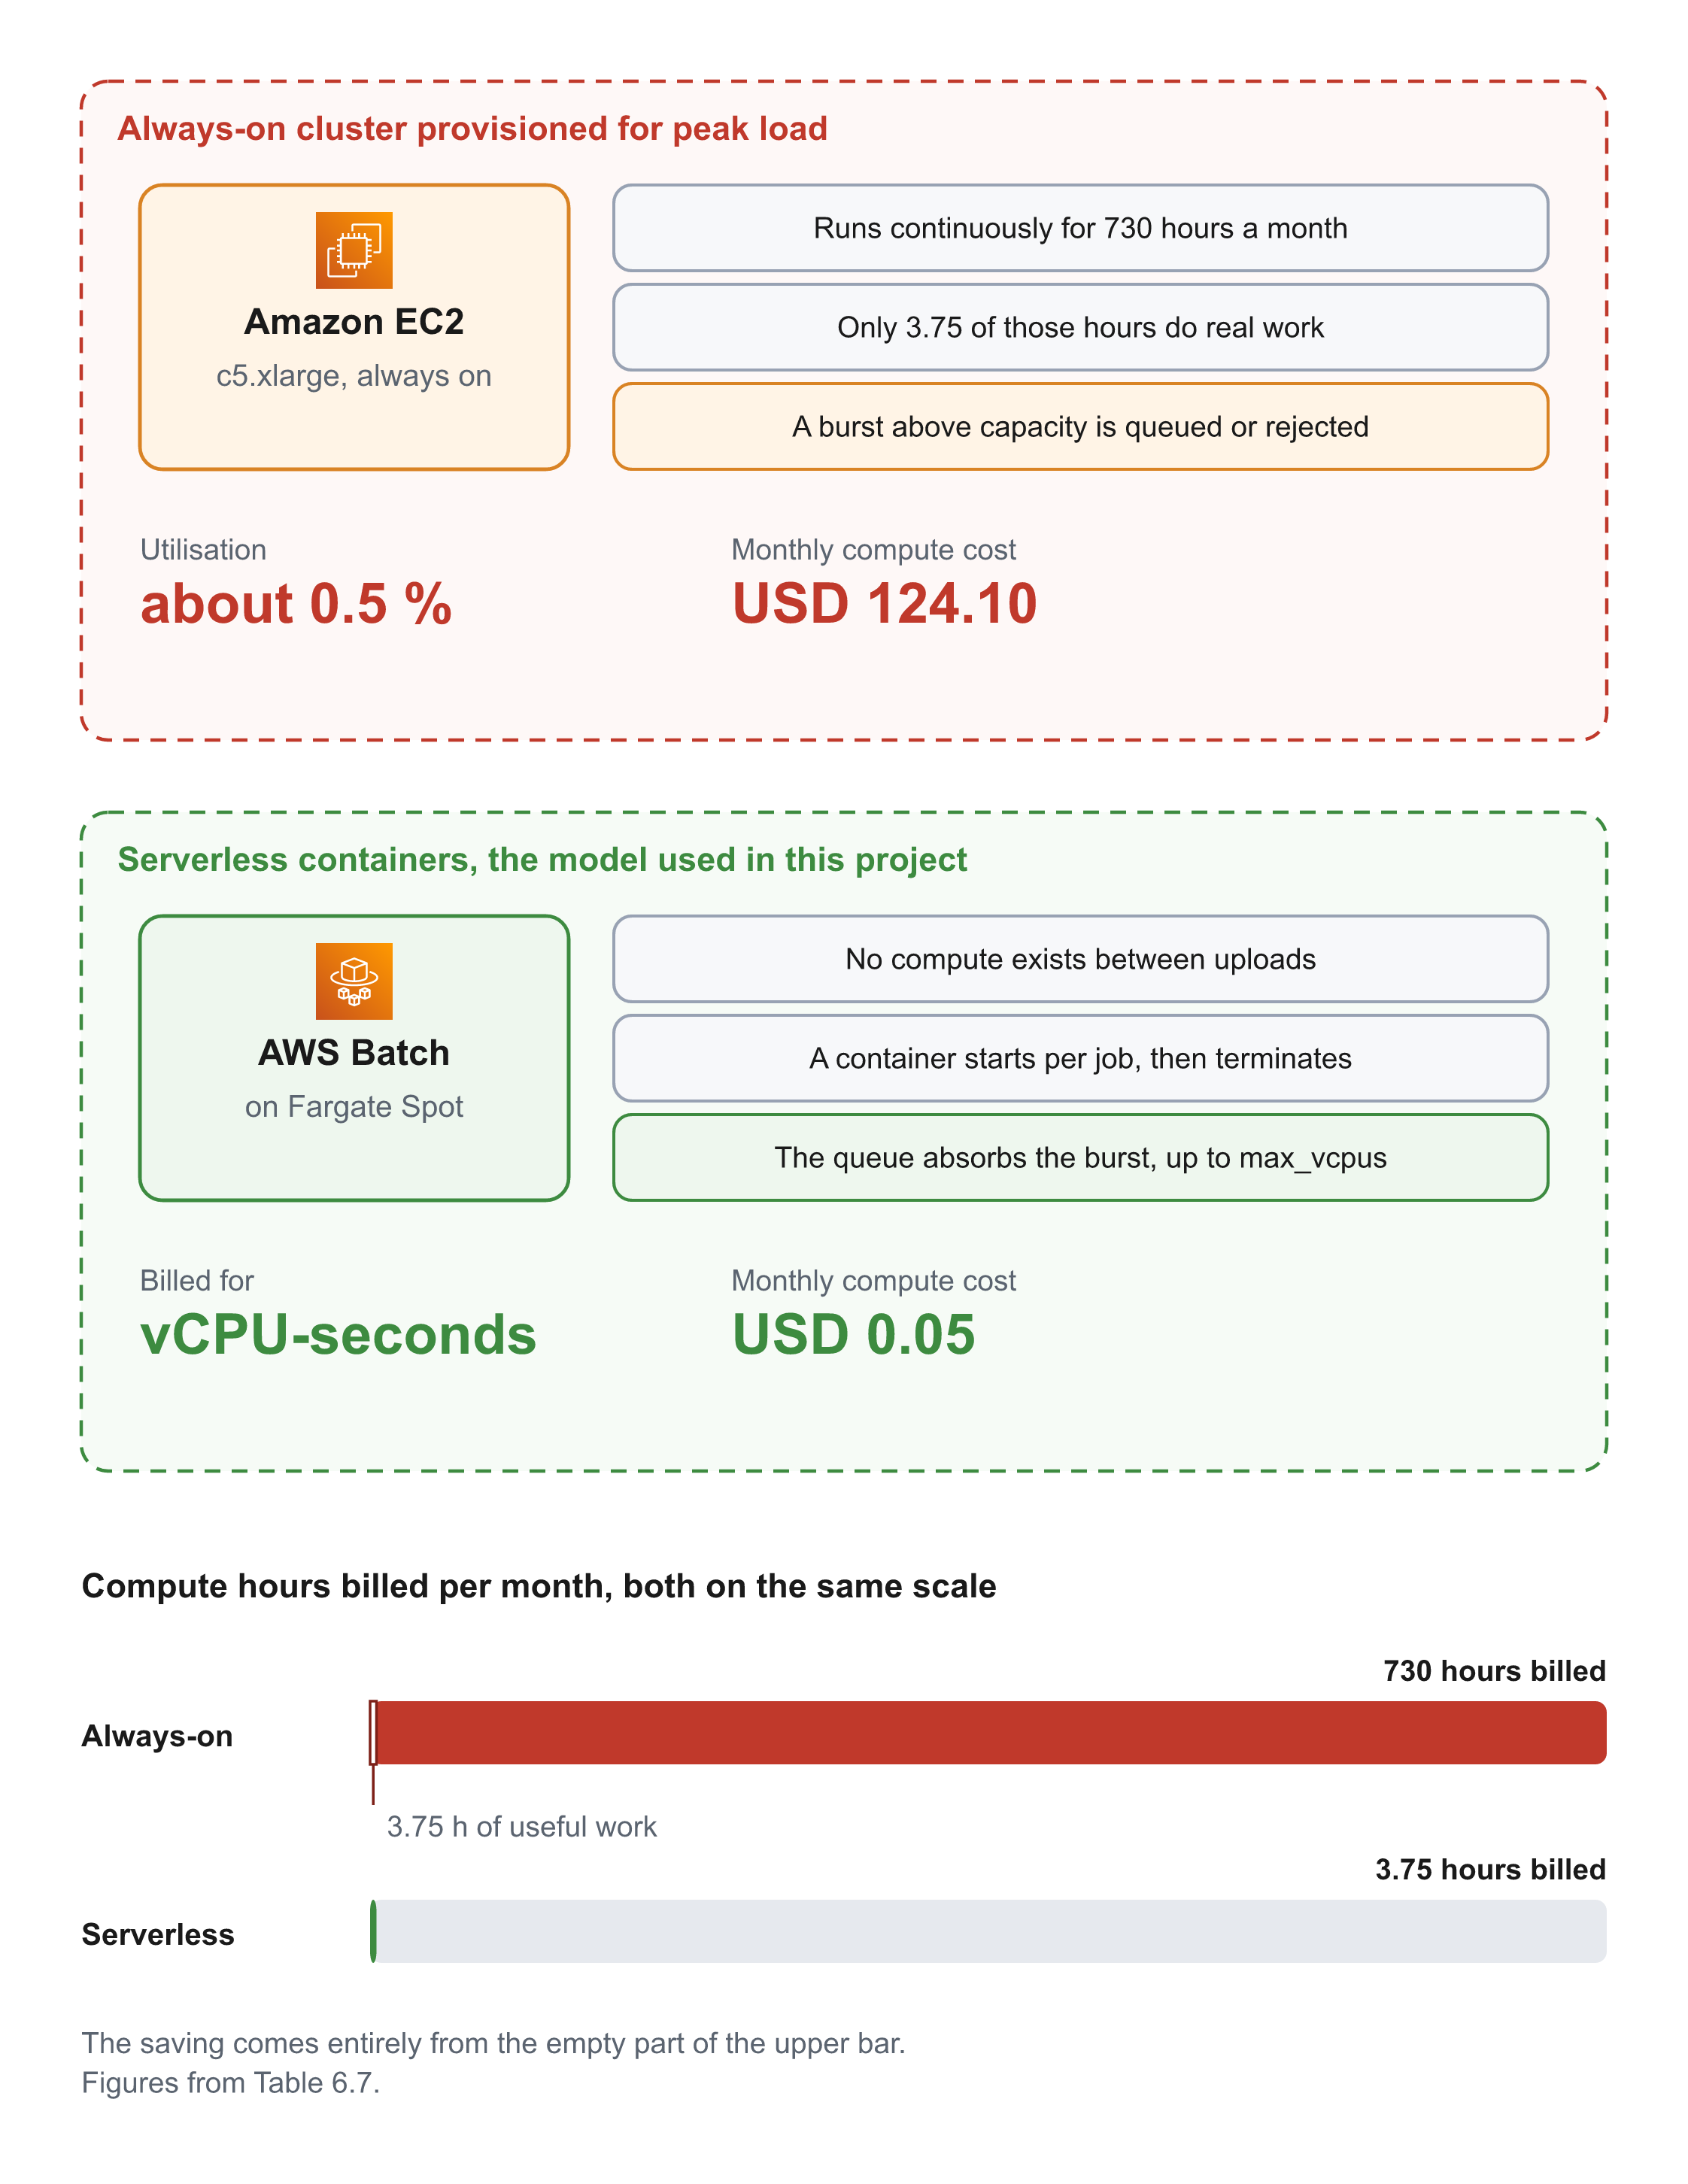
\includegraphics[width=0.82\textwidth]{images/07-compute-models.png}
\caption{\textit{Compute models for a bursty transcoding workload: an always-on cluster
compared with on-demand serverless containers}}
\label{fig:compute-models}
\end{figure}

The choice of Fargate over a function-as-a-service platform such as AWS Lambda deserves
justification, because Lambda is the more common answer to serverless workloads. Video
transcoding is unsuitable for Lambda in this context for two reasons. The first is duration:
transcoding a large file routinely exceeds the maximum execution time of a Lambda invocation.
The second concerns resource configuration. A measurement study of serverless video processing
found that selecting a cost-efficient memory configuration for transcoding is far from trivial,
because the optimal setting depends not only on the type of task but even on the content of the
video itself, and the cost difference between the least and most generous memory configuration
reached 498\% for sequential workloads \cite{nossdav2019video}. Fargate avoids this
difficulty by allowing vCPU and memory to be specified explicitly and independently.

A known weakness of the container model is cold start latency. A systematic review of the
subject reports that more than half of function invocations spend at least 80\% of their
startup time pulling the container image \cite{coldstart2023}. This finding directly motivates
the use of a multi-stage Docker build in this project, described in
Section~\ref{sec:transcoder-impl}, whose purpose is to minimise the size of the image that must
be transferred before work can begin.

\subsection{Event-Driven Architecture}

An event-driven architecture propagates work through the emission and consumption of events
rather than through direct synchronous invocation. In this project, the completion of an upload
to Amazon S3 emits an event notification that is placed on an Amazon SQS queue, from which an
AWS Lambda function submits a job to AWS Batch.

The queue is not merely a routing mechanism; it is the component that makes burst absorption
possible. If a hundred users upload simultaneously, the queue retains all hundred messages
while AWS Batch works through them at whatever rate the compute environment allows. Without
this buffer, the system would have to either reject work or provision for peak load
permanently. The queue is paired with a dead letter queue so that messages which repeatedly
fail processing are isolated for inspection rather than being retried indefinitely.

\subsection{Adaptive Bitrate Streaming and the Bitrate Ladder}

HLS delivers a video as a master playlist referencing several rendition playlists, each of
which lists the media segments for one quality level. The player measures throughput and
switches between renditions at segment boundaries.

Figure~\ref{fig:hls-abr} shows the artefacts this produces and the order in which a player
retrieves them. A single source file of arbitrary container, codec and resolution is encoded once
per rung of the ladder, and each rung yields both a rendition playlist and the sequence of
transport stream segments it indexes. The master playlist sits above them and carries, for each
rung, the bandwidth the client should expect to need in order to play it. A player therefore
begins by fetching only the master playlist, which is a few hundred bytes, chooses a rung from the
declared bandwidths and its own throughput estimate, and only then requests that rung's playlist
and its segments. Because every rung is segmented on the same boundaries, the player may change
its choice at any segment boundary without interrupting playback, which is the mechanism that lets
quality fall rather than the video stall when a connection weakens. The consequence for the
transcoding subsystem is that the cost of preparing a video scales with the number of rungs, since
each rung is encoded separately even though the source itself is decoded only once. The
implementation exploits exactly that distinction, as Section~\ref{sec:transcoder-impl} describes.

\begin{figure}[H]
\centering
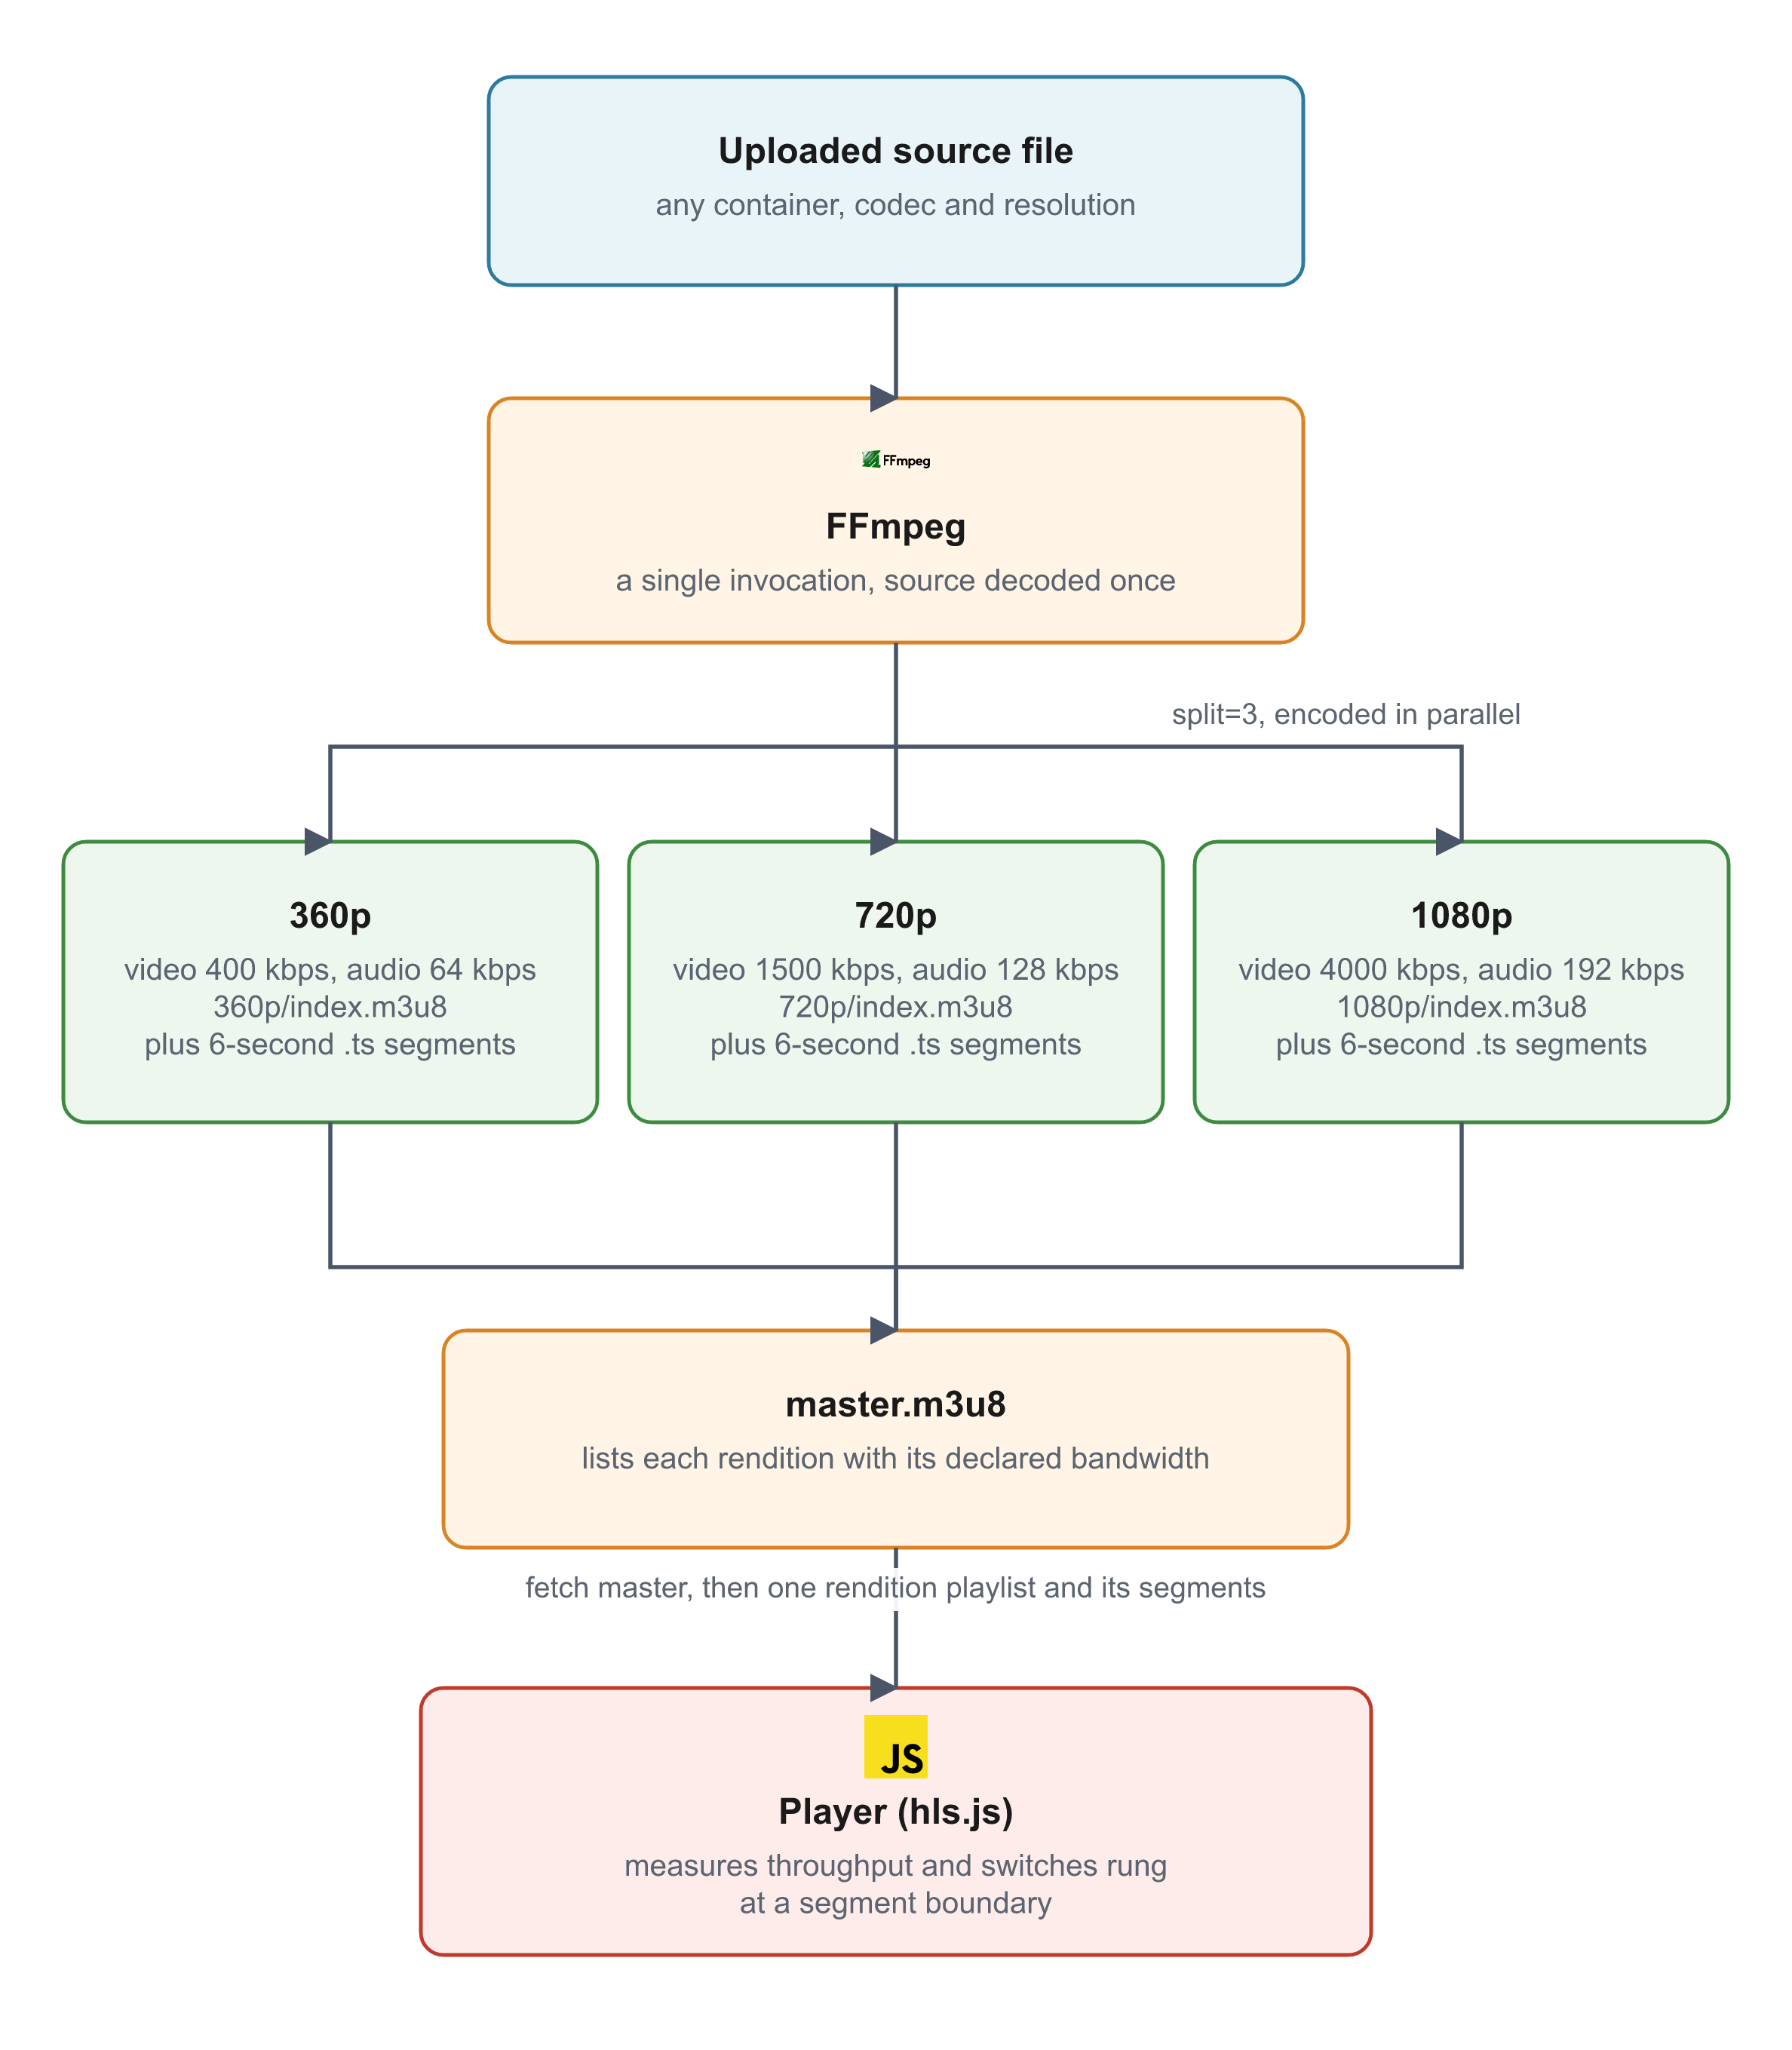
\includegraphics[width=0.85\textwidth]{images/06-hls-abr.png}
\caption{\textit{HLS artefacts produced from one source file and the order in which a player
retrieves them}}
\label{fig:hls-abr}
\end{figure}

The set of resolution and bitrate pairs offered is called the bitrate ladder, and its
construction is an active research area. Netflix demonstrated that the optimal ladder is not
fixed but content-dependent, and that the ideal operating points lie on the convex hull of the
quality-versus-bitrate curve \cite{netflix2015pertitle}. By encoding each shot separately under
the control of the VMAF perceptual quality metric, Netflix reported bitrate reductions of
between 28\% and 38\% at equivalent visual quality \cite{netflix2018dynamic}. The present
project uses a fixed three-rung ladder, which is simpler to implement and reason about; the
implications of this simplification are revisited in Section~\ref{sec:future-work}.

\section{Technology Stack Justification}
\label{sec:tech-stack}

The frontend is implemented as a React single page application built with Vite, using HLS.js
for playback. HLS.js is necessary because most desktop browsers do not support HLS natively;
it parses the manifest in JavaScript and feeds segments to the browser through the Media Source
Extensions API. Safari, which does support HLS natively, is handled through a fallback path.

The backend is built on Node.js with Express. The decisive factor is that the backend's
workload is almost entirely input/output bound rather than CPU bound: it issues pre-signed
URLs, queries MongoDB, and returns JSON, while the heavy computation is deliberately delegated
to the transcoder containers. Node.js's event loop is well suited to this profile.

MongoDB Atlas provides the persistence layer. Video metadata is naturally document-shaped and
its schema evolves as features are added, which suits a document store better than a rigid
relational schema. Using the managed Atlas service also removes the need to operate a database
cluster inside the project's own infrastructure.

Terraform was selected for Infrastructure as Code over alternatives such as AWS CloudFormation
because its module system allows the infrastructure to be decomposed into reusable units with
explicit inputs and outputs, and because its plan step makes the consequences of a change
visible before it is applied. GitHub Actions was selected for CI/CD because the source code is
already hosted on GitHub, which removes the need for a separate automation server.
